\section{Experiments}

\subsection{Experiment Settings}
Generally \(3\) data sets (\emph{abalone}, \emph{bodyfat} and \emph{housing}) are 
chosen to test the optimization methods. For all datasets, \(80\%\) data is used for
training and remaining data is used for testing. In order to improve the performance,
the scaled data is used.

First I build up the linear model using C++ which can be find in LinearModel.h and 
LinearModel.cpp. Before training, the weights of this linear model are initialized
randomly.

Then three optimization methods are implemented in Optimizer.h and Optimizer.cpp.
For all methods, the stop criteria are designed based on the 
\emph{first-order optimality condition}: the iteration will last untill the gradient 
of objective function is small enough (\(\grad f(\xB) \le \varepsilon\)). Here I set
\(\varepsilon\) to \(10^{-10}\).

For the rigde regression expressed in Equation.~\ref{eq:beta-rigde}, I choose 
\(\lambda = 0.0, ~0.1, ~0.5, ~1.0, ~5.0, ~10.0\) to test the optimization methods.
For all optimization methods, step sizes are chosen according to Theorem.~\ref{thm:step-minimizer}.

In the whole work, the Eigen library is used to perform matrix operations.

\subsection{Experiment Results}
The MSE losses on testing dataset of three optimization methods are shown in Fig.~\ref{fig:grad}, Fig.~\ref{fig:conjgrad}
and Fig.~\ref{fig:qn}. From three figures we can find that Conjugate Gradient Methods and Quasi-Newton Methods 
converge much more quickly than Gradient Method. Even though for all algorithms we choose the best step size during the iterations,
Gradient Method still needs more than \(10000\) iterations to reach designed accuracy. From these experiments we can compare the rate
of convergence of three methods directly, and this also satisfies analysis.

\begin{figure}[!htbp]
    \centering
    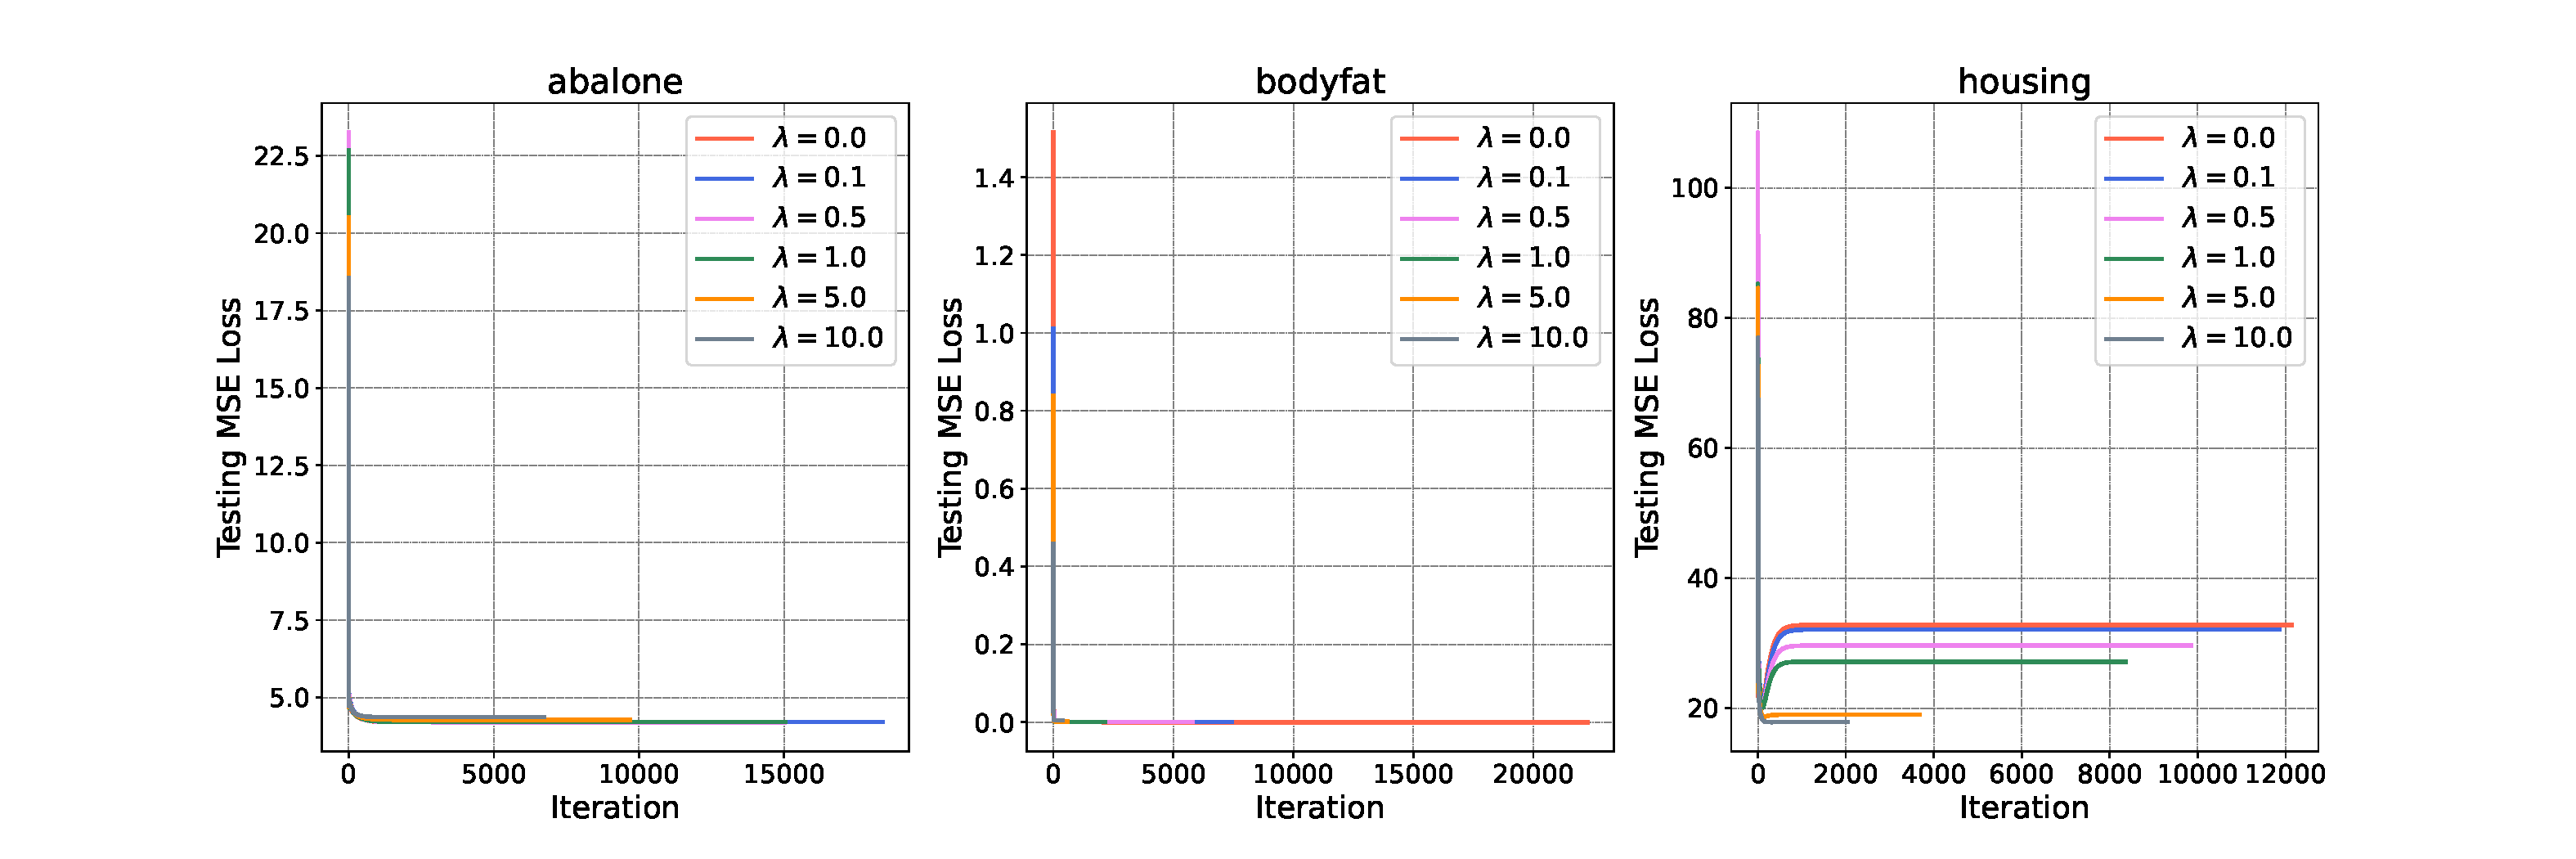
\includegraphics[scale = 0.28]{fig/Grad.pdf}
    \caption{Testing MSE Loss of Gradient Methods on \(3\) datasets.}
    \label{fig:grad}
\end{figure}

\begin{figure}[!htbp]
    \centering
    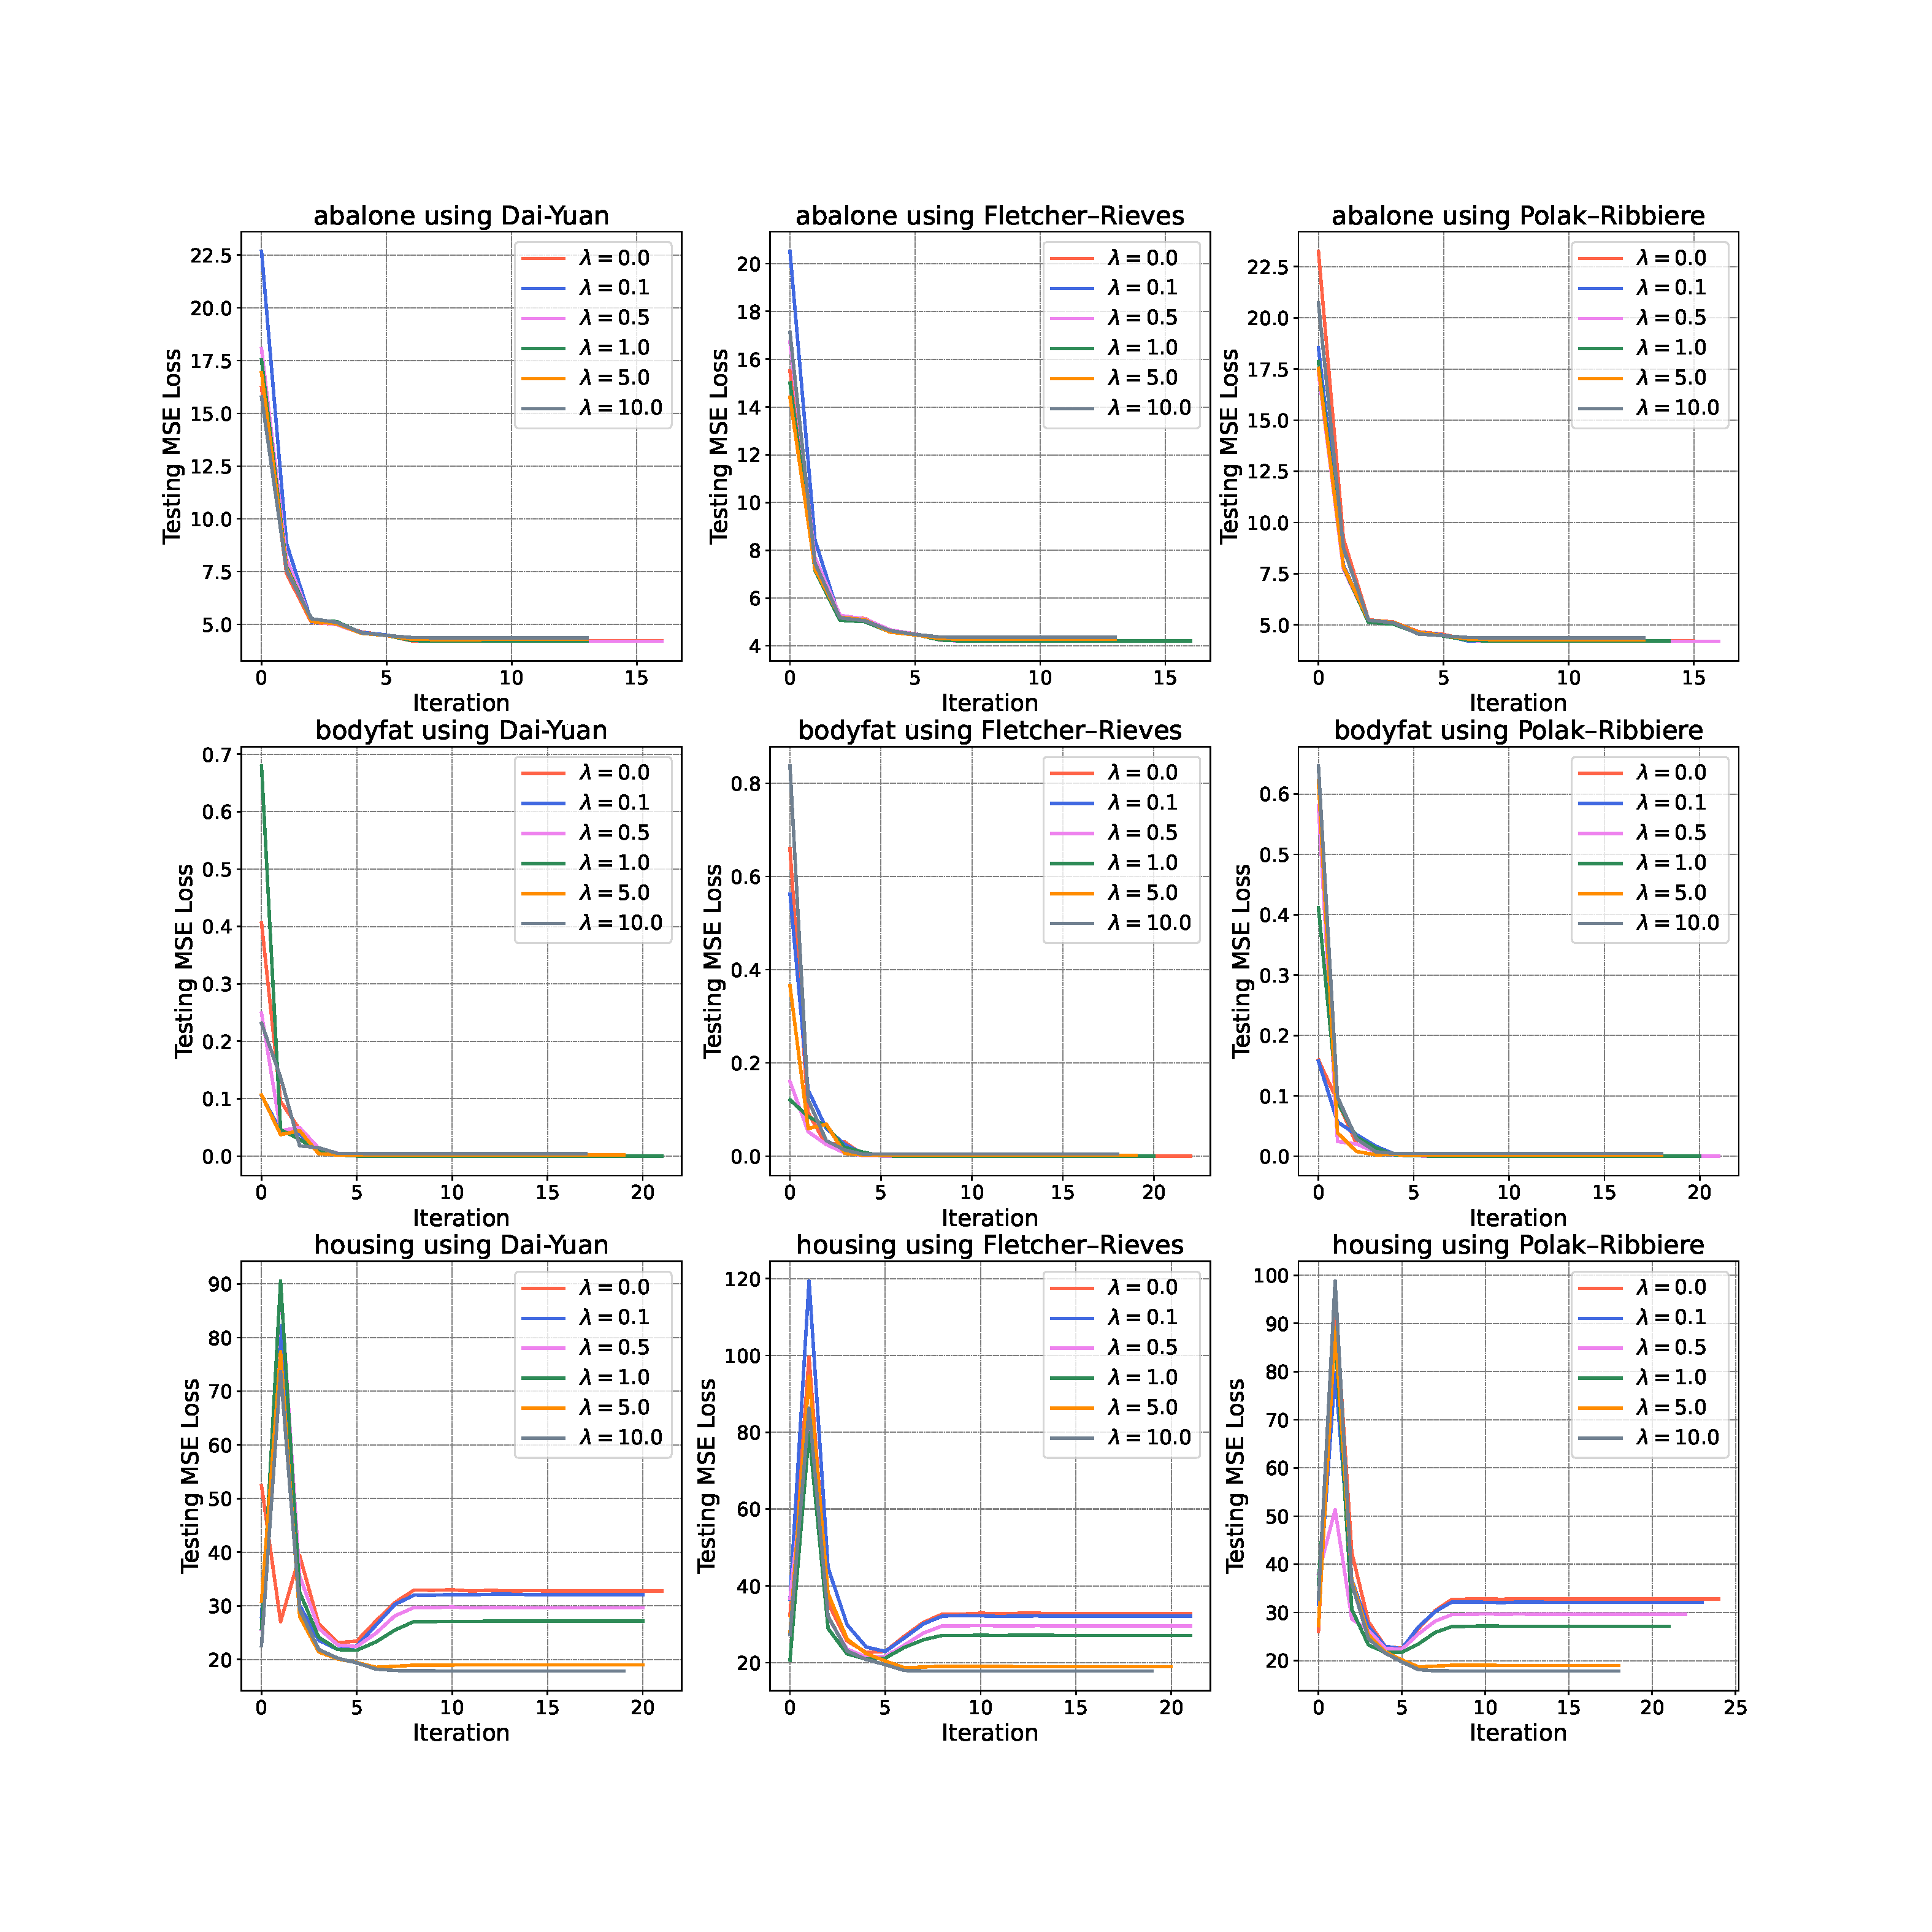
\includegraphics[scale = 0.28]{fig/ConjGrad.pdf}
    \caption{Testing MSE Loss of Conjugate Gradient Methods on \(3\) datasets.}
    \label{fig:conjgrad}
\end{figure}

\begin{figure}[!htbp]
    \centering
    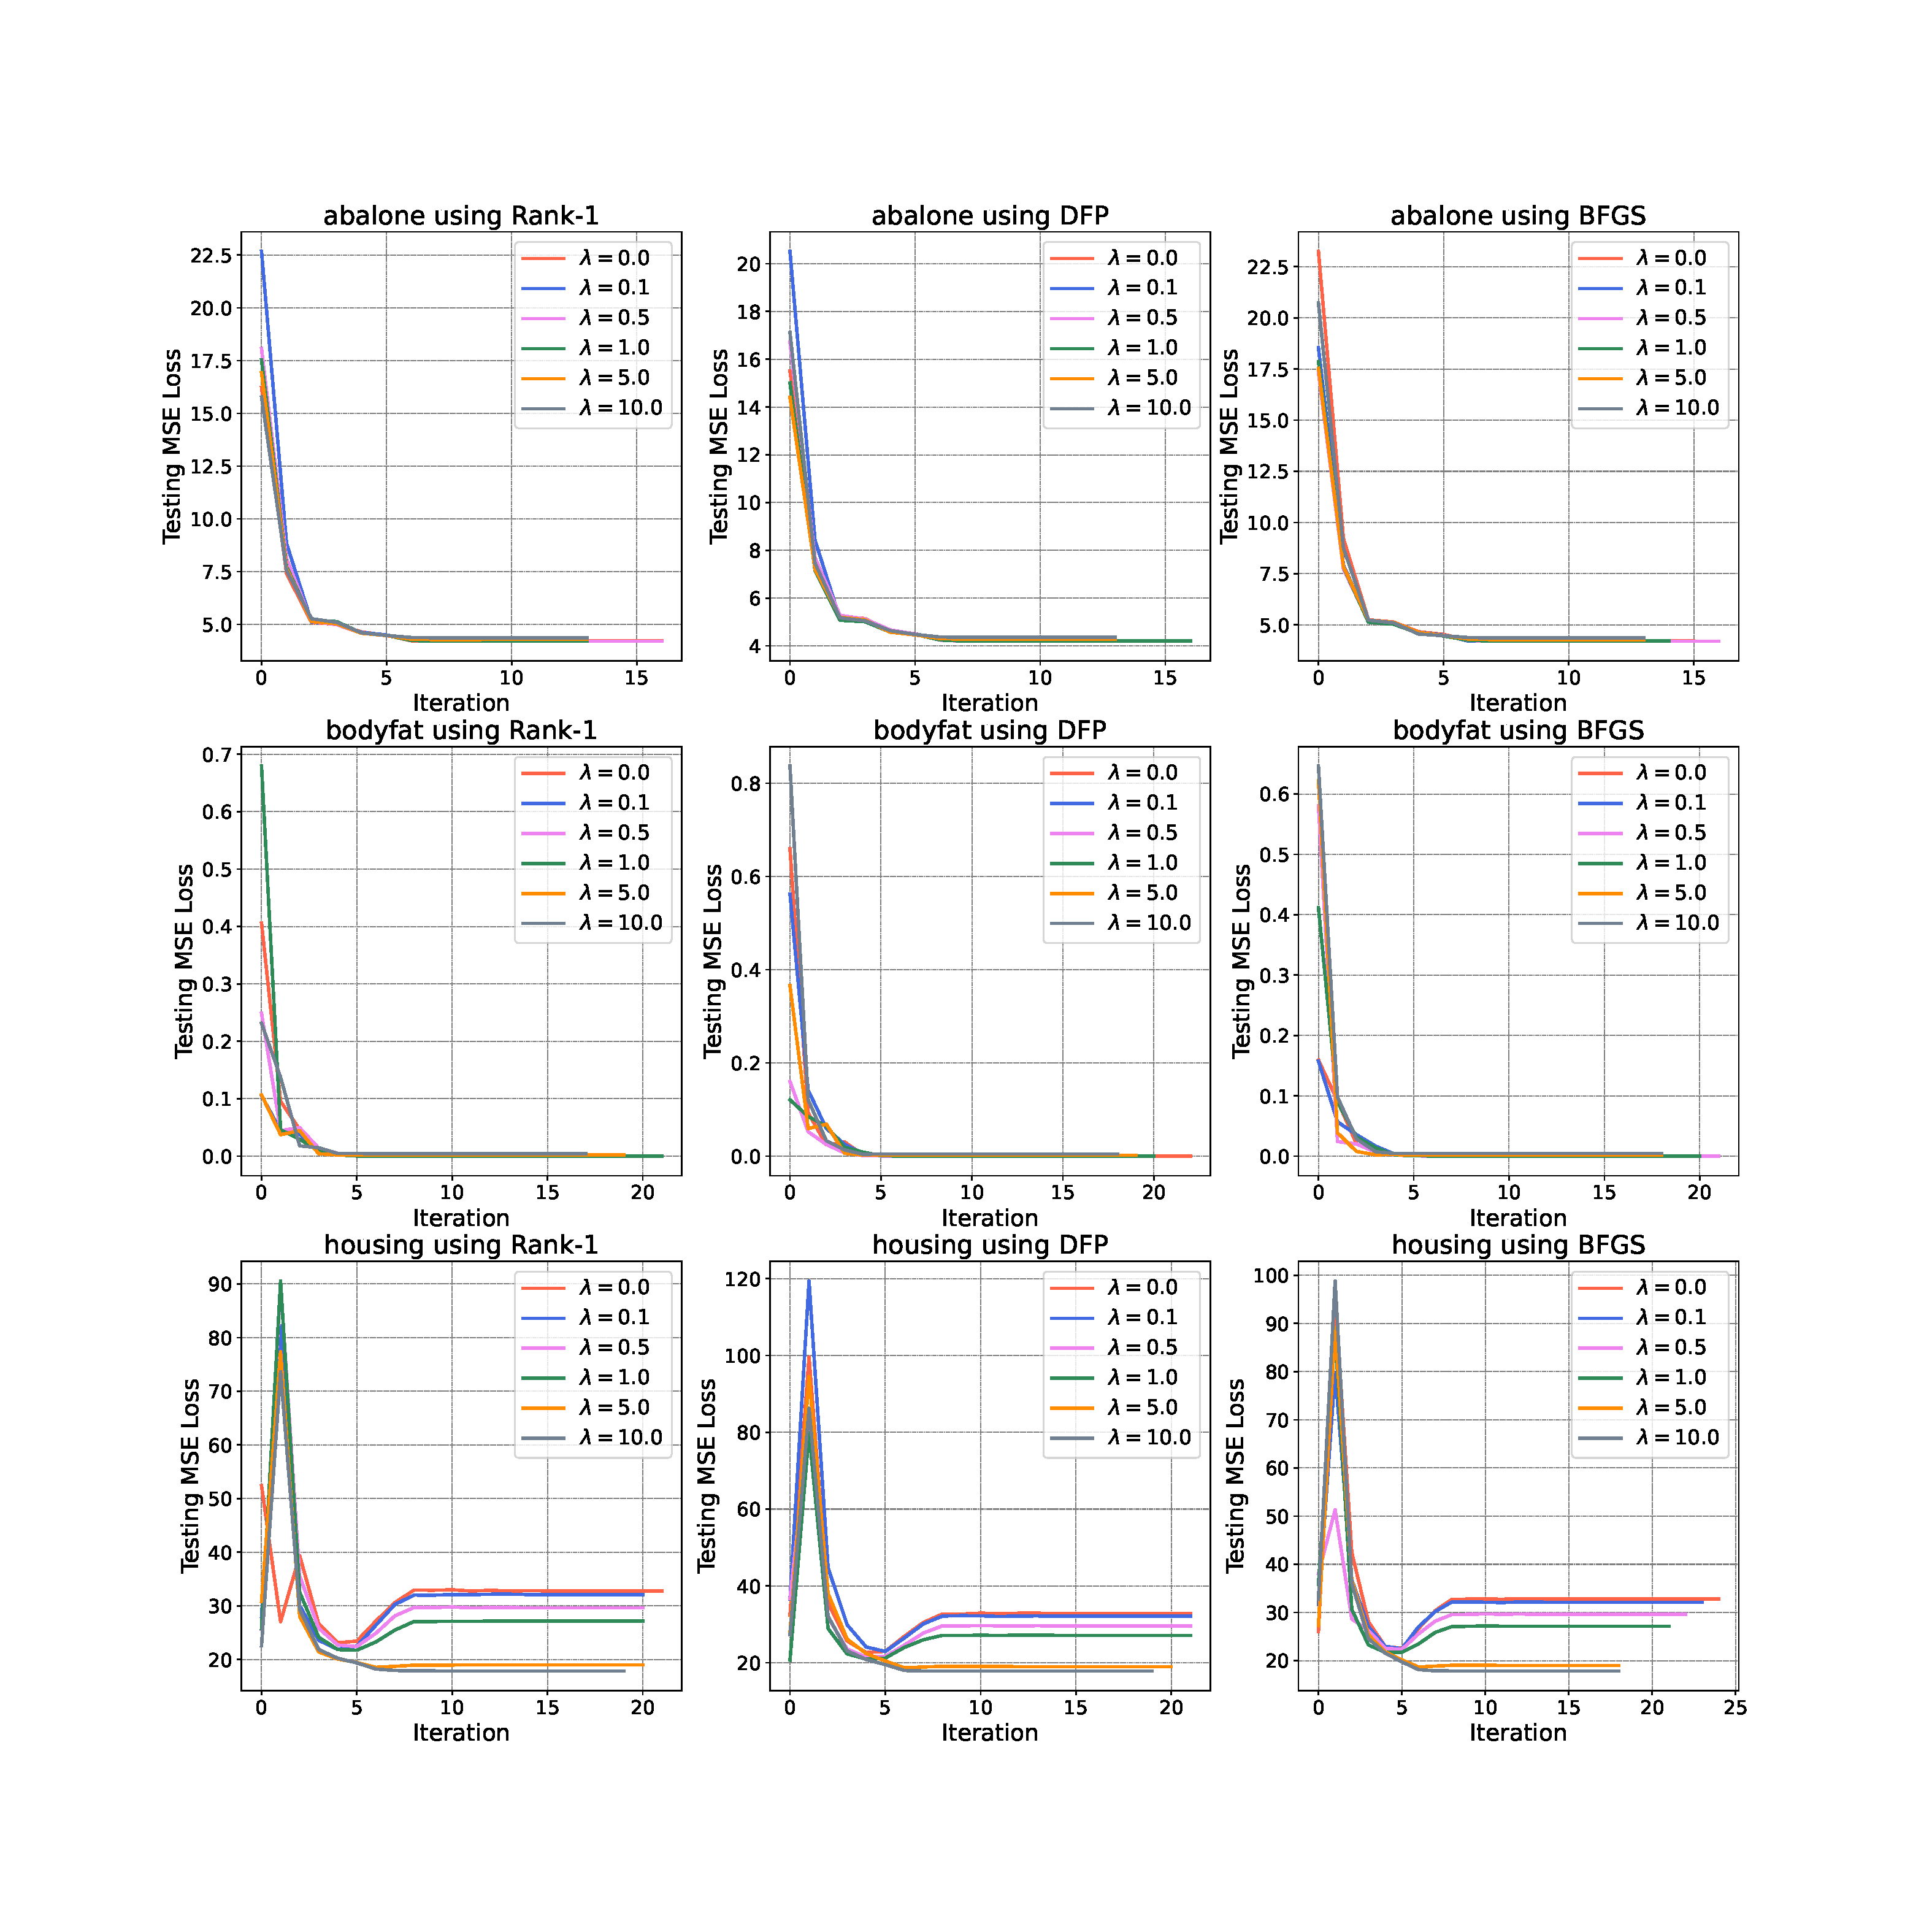
\includegraphics[scale = 0.28]{fig/QN.pdf}
    \caption{Testing MSE Loss of Quasi-Newton Methods on \(3\) datasets.}
    \label{fig:qn}
\end{figure}